\section{Proactive Curiosity and Questions}
\label{sec:curiosity}

A key claim of this paper is that a personal AI should improve by forming a
small, correctable understanding of the person, not by accumulating free-form
memory notes. Elephant Agent treats memory as a five-layer architecture:
Personal Model, Elephant State, Episode / Loop / Step trail, Contextual Recall,
and Background Learning. Within that architecture, the durable Personal Model
has two objects: \texttt{Fact} and \texttt{Question}.

\begin{figure}[t]
  \centering
  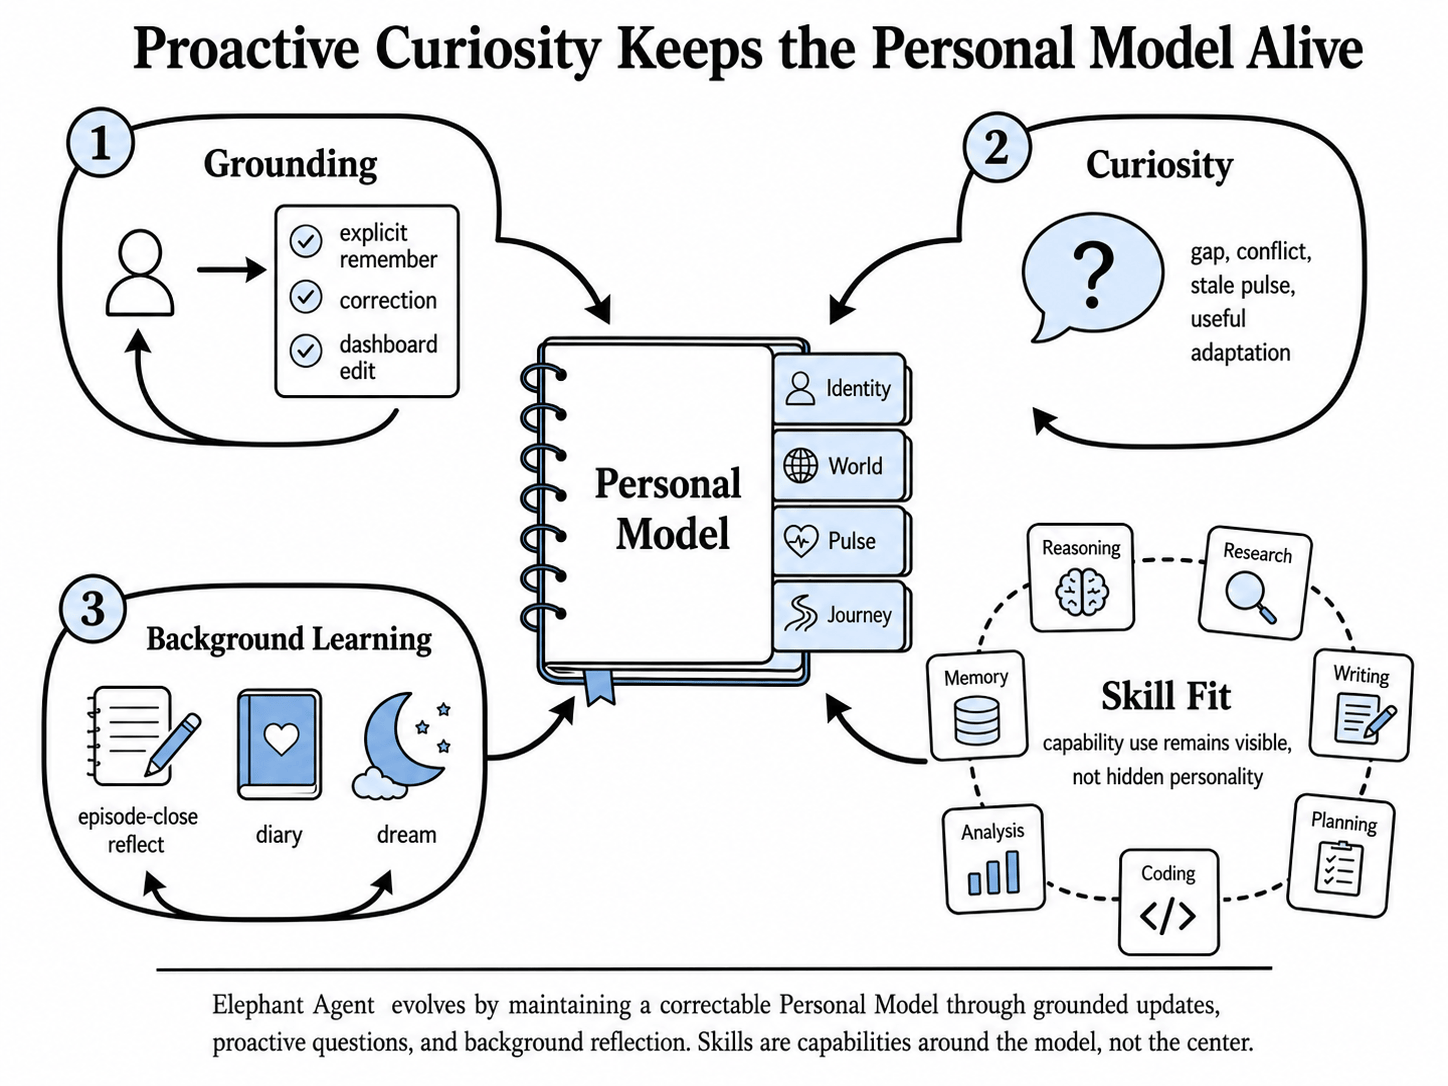
\includegraphics[width=0.9\linewidth]{../../apps/site/static/assets/resources/paper-5.png}
  \caption{Proactive curiosity keeps the Personal Model alive through grounded
  user updates, bounded questions, background learning, and visible skill use
  around the model rather than hidden personality changes.}
  \label{fig:proactive-curiosity-loop}
\end{figure}

\subsection{Facts}

A \texttt{Fact} is the smallest unit of Personal Model truth. Every fact has a
reference, lens, topic, text, status, confidence, source, and
\texttt{source\_episode\_ids}. Statuses are \texttt{active}, \texttt{retired},
and \texttt{disputed}. Only active facts enter the stable prompt.

\begin{description}
  \item[\textit{Identity}] Stable self-description, values, decision style,
  boundaries, and durable preferences.
  \item[\textit{World}] People, relationships, projects, tools, places,
  vocabulary, domains, and stable surrounding context.
  \item[\textit{Pulse}] Current work, current life phase, active pressure,
  recent constraints, priorities, and temporary mood or energy patterns.
  \item[\textit{Journey}] Lessons learned, past experiences, recovery patterns,
  repeated failures, decisions, and long-running growth trajectory.
\end{description}

\subsection{Provenance}

Provenance explains why a fact exists. It is not a separate durable storage
layer. It lives in the entities that reference source material:
\texttt{Fact.source\_episode\_ids}, Step records, and SemanticIndexEntry rows.

When the user asks why Elephant Agent believes something, Elephant Agent traces source Episode
ids, loads relevant Steps, and presents the support material. The support can
help the current turn or inspection flow, but it is not itself prompt truth.

\subsection{Proactive Curiosity and Questions}

A \texttt{Question} is a lens/topic-bound attempt to improve future help. Elephant Agent
creates questions for four reasons only: an important gap, a conflict, a stale
Pulse claim, or a high-value adaptation that would materially change future
behavior. Questions are not a profile-filling checklist.

The product behavior is proactive curiosity rather than a question engine.
Elephant Agent can actively maintain understanding at a user-selected effort level:
\textit{quiet} mostly waits and asks rarely, \textit{balanced} asks at natural
pauses when the answer would help, and \textit{active} is more willing to check
in while still staying optional. These levels govern frequency and willingness
to communicate, not autonomous task execution.

When Elephant Agent asks a question, the lifecycle is explicit: the question moves from
\texttt{open} to \texttt{asked}; the user's answer marks it \texttt{answered};
and the answer is applied through the same Personal Model update path as any
other durable fact. A dismissed question stays visible as a boundary rather
than being re-asked silently. Silence is honored at every effort level.

\subsection{Foreground Tools}

The model-facing surface is deliberately small:

\begin{itemize}
  \item \texttt{tool.personal\_model.search} reads active facts and optional
  provenance.
  \item \texttt{tool.personal\_model.update} is the only foreground write path
  for durable understanding. It supports \texttt{remember}, \texttt{correct},
  \texttt{forget}, and \texttt{dispute}.
  \item \texttt{tool.personal\_model.questions} manages question list, ask,
  answer, and dismiss actions.
\end{itemize}

There is no \texttt{tool.memory.note} in the clean design. Memory is not a
free-form foreground write surface. Current-turn recall is the retrieval layer;
durable understanding changes only through Personal Model tools.

\subsection{Prompt Projection}

Stable prompt projection contains only Elephant identity, active four-lens facts,
the Episode opening resume snapshot when available, and tool policy.
Current-turn retrieval is injected separately as \texttt{Current-turn recall support:}; it is
support for the current turn, not a source of durable truth. Retired facts,
disputed facts, raw memory entries, semantic index rows, and style summaries
are not projected as stable understanding.

\subsection{User Visibility}

The dashboard You page shows the four lenses directly. Each fact can be
corrected, forgotten, or inspected through a \textit{Why} expansion. The
Questions page shows open, asked, answered, and dismissed Personal Model
questions and links answered questions to the facts they produced. This makes
learning inspectable: Elephant Agent does not silently model the user; it maintains a
small set of facts the user can challenge.
